\chapter{Generalizing the Earth Mover's Distance for Efficient Neural Network Regularization} \label{chap:demd}
Selections of parameters related to individual samples can help with single sample problems,
but the majority of learning problems are more concerned with generalization: if a subset of samples known to be related are behaving differently, can we identify them, and can we remove this difference?
Here, we aim to account for groups of samples that behave differently compared to others, and efficiently regularize models toward fairer solutions.


Optimal transport (OT) has emerged as useful tool for a wide range of applications including information retrieval \citep{balikas2018cross,yurochkin2019hierarchical}, image processing \citep{otip}, statistical machine learning, as well as more recently, for applications in ethics and fairness \citep{kwegyiraggrey2021relative}. 
OT is especially well-suited for tasks where dissimilarity between two or more probability distributions must be quantified,
and its success has been made possible through dramatic improvements in numerical algorithms \citep{cuturi2013sinkhorn,solomon2015convolutional} that allow one to efficiently optimize commonly used functionals.
In practice, OT is often used to estimate and minimize the 
the distance between distributions of interest, 
and this is done using an appropriately defined loss functional. %Recent advances provide us the capability to drop-in and seamlessly integrate many types of losses into existing methods, for novel applications.

%\begin{comment}
%\vikas{the following paragraph is low on content. Perhaps take 1-2 initial lines, compress and use it close off the previous paragraph?}
%The driving practical focus of optimal transport aims to estimate and minimize the distance between distributions of interest. Within machine learning, this takes the form of a loss; recent developments have enabled constructions of such a loss that allow almost seamless integration into existing methods. These incorporations have led to a number of benefits over traditional mean-squared error approaches, taking direct advantage of the statistical and distributional assumptions and requirements of the model fitter.
%\end{comment}

{\bf Barycenters.} 
%{\color{red}Can next two paragraphs merge? Start this with "One way to quantify dissimilarity between many distributions is through distance to the mean....  "} While distances are defined between two points (or two probability distributions), barycenters extend the idea and enable analyzing many points (or probability 
One way to quantify dissimilarity between many distributions is through distance to the mean. Here, for averaging,  
we measure pairwise distances.
Practically, this has led to models that can 
concurrently enforce distributional similarity between a 
set of distributions and has found use in 
a spectrum of applications.

\begin{figure*}[ht]
    \centering
    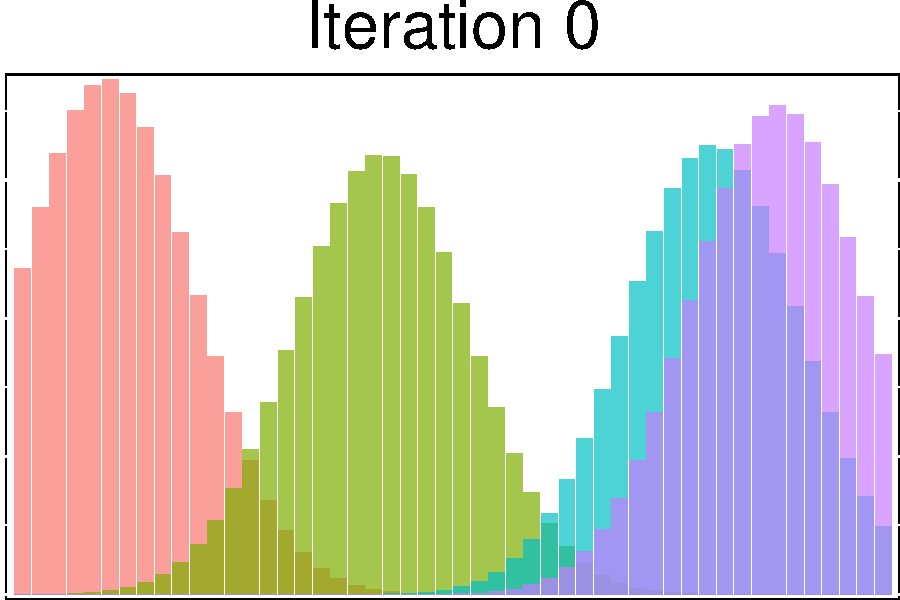
\includegraphics[width=0.19\textwidth]{chap5/hists/hists_iter_0.pdf}
    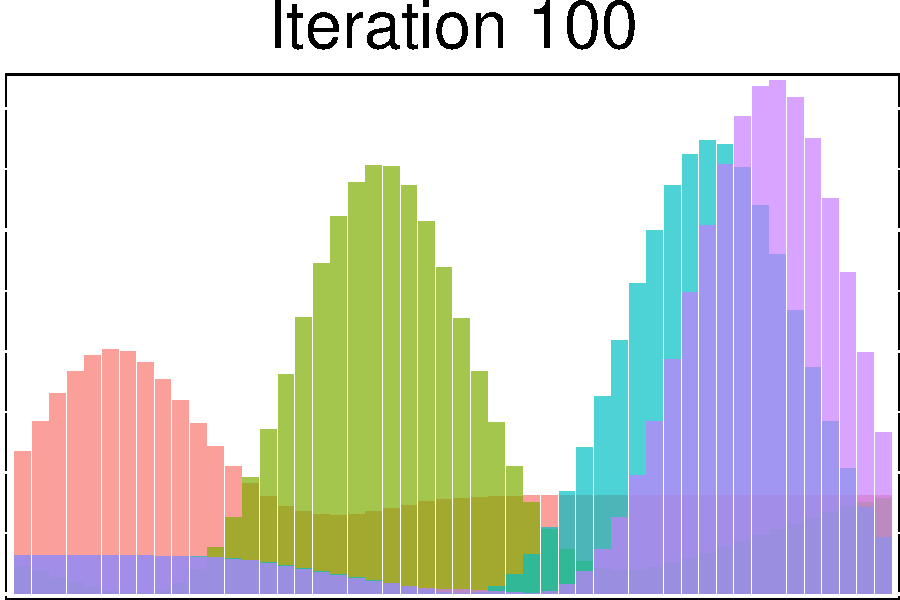
\includegraphics[width=0.19\textwidth]{chap5/hists/hists_iter_100.pdf}
    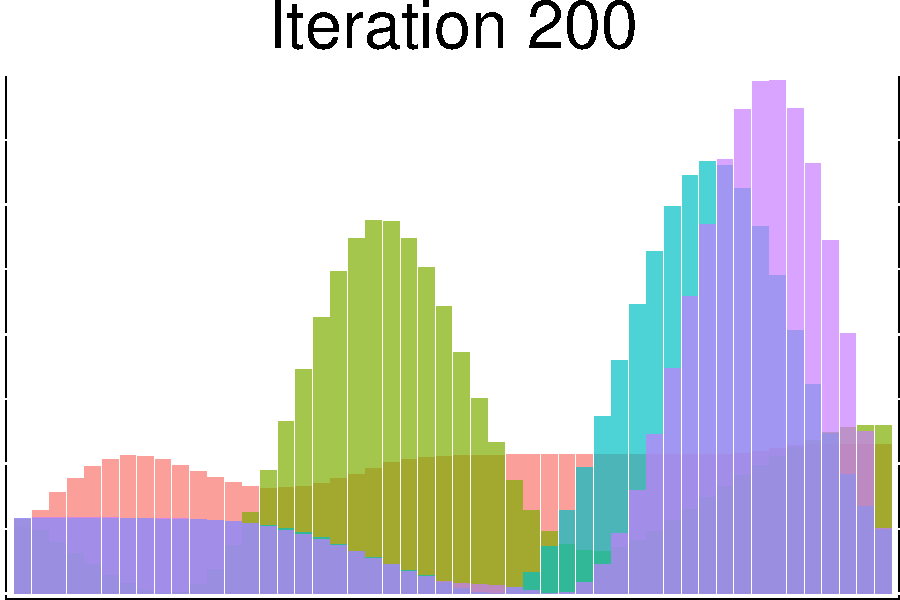
\includegraphics[width=0.19\textwidth]{chap5/hists/hists_iter_200.pdf}
    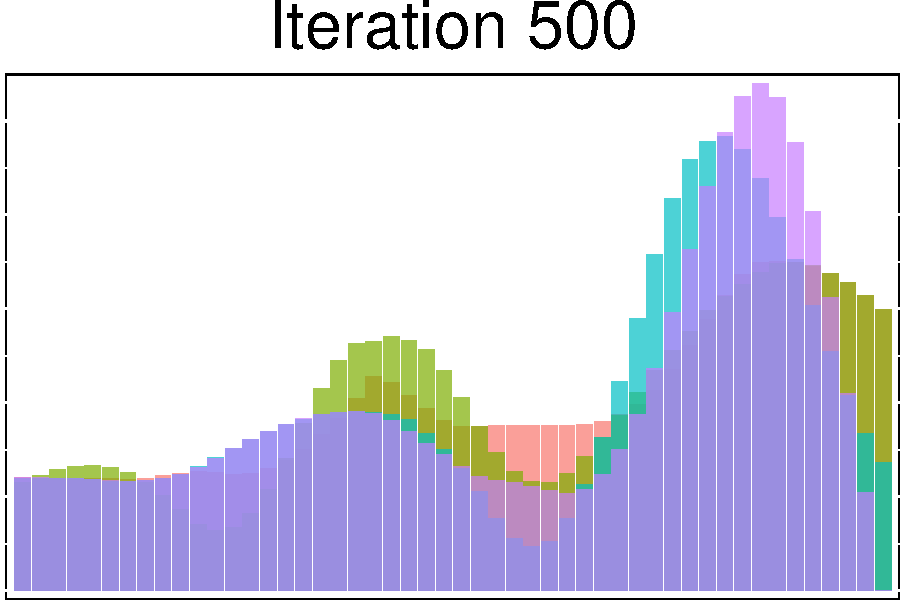
\includegraphics[width=0.19\textwidth]{chap5/hists/hists_iter_500.pdf}
    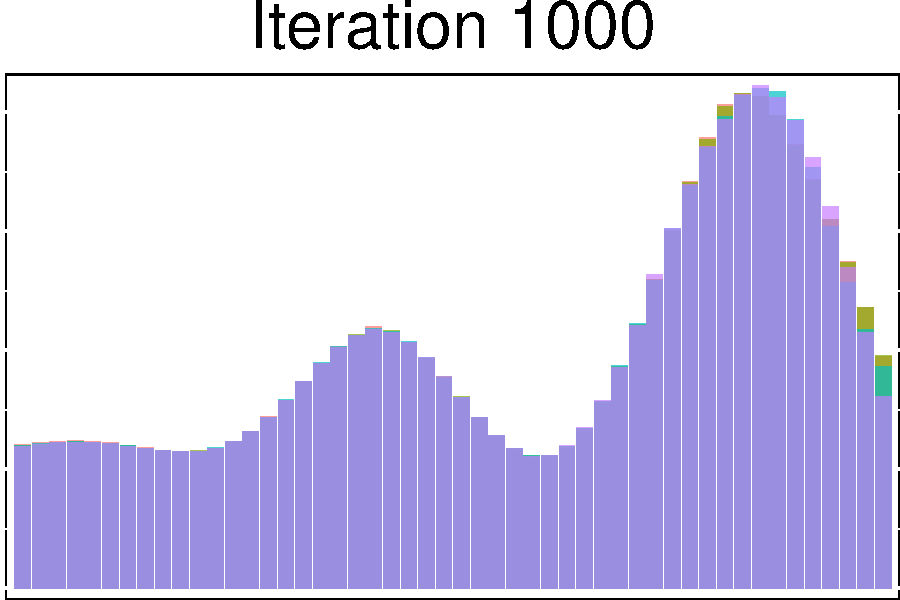
\includegraphics[width=0.19\textwidth]{chap5/hists/hists_iter_1000.pdf}
    \caption{This figure shows the starting and ending state of an iterative process applied to 4 histograms. Each iteration minimizes the generalized Earth Mover's objective, and then updates each histogram in the direction provided by the gradient. Upon each iteration shifts a portion of ``mass'' of every histogram closer to a common distribution. ({\em Left}) The process initially starts with $d=4$ histograms with 50 bins each. ({\em Right}) The update process eventually converges. An intuitive description is that the mass of the original 4 histograms is incrementally shifted around at each step, and all four distributions eventually are reshaped into the limiting distribution, which appears at right. }
    \label{fig:hists}
\end{figure*}

%{\bf Barycenter calculation.} 
Assuming that a suitably regularized form of the optimal transport loss is utilized, the pairwise distance 
calculation is efficient -- in fact, 
in some cases, Sinkhorn iterations can be used \citep{cuturi2013sinkhorn}. 
On the other hand, to minimize distances to the mean, 
most algorithms typically operate 
by repeatedly estimating the barycenter and those pairwise distances, and using a ``coupling'' strategy 
to push points toward the barycenter. 
The idea is sensible but as the number of distributions 
grows, the overall procedure becomes 
computationally intensive.
For example, even on a high end workstation, 
simply computing the barycenter over
50 distributions with 50 bins
%does not converge within a reasonable number of iterations
%using newer packaged solvers. {\color{red} maybe instead of ``not...reasonable'', try ``not competitive"}
proves to be a time-intensive process.
However, very recent research has shown that there exist polynomial time algorithms for this problem 
%have been shown to exist within the last year
\citep{altschuler2021wasserstein}. 
% \vikas{can we concretize it 
% a little more? cite some numbers on a standard workstation? memory requirements? other resource needs?}
 %{\color{red} Glenn: fairness lead}

% {\color{red}this para does not add much}
% Importantly, we should also appreciate that the calculation of the barycenter is often a means to an end in most learning applications -- 
% the ultimate goal tends to be pushing these distributions to come closer. 
% A barycenter is a modeling choice, but other options may also be viable. 
% Indeed, if a different global measure of ``distributional disparity''
% were to be defined and minimized, the costs associated with pairwise comparisons and optimization
% may potentially be avoided. This hypothesis drives much of our development.

\noindent\textbf{Where can we measure dissimilarity?}
% {\color{red} START} Putting aside the cost to compute the barycenter for the moment, 
% instantiations of such applications often desire to enforce distribution similarity
% only on model outputs.
% For example, in \citep{jiang2020wasserstein}, the authors define fairness measures over the probability of the prediction given ground truth labels.  
% This choice is not without good reasons: discrete outputs lead to extremely nice distributions over the probability simplex, where optimization is easy and assumptions need not be strong.{\color{red} END; could START--END be replaced with the gray text?}
In applications, it is often a goal to enforce distribution similarity on model outputs. For example, in \citep{jiang2020wasserstein}, the authors define fairness measures over the probability of the prediction given ground truth labels.   
%FIXME: if you read this and know what X Y and Z are, then fill in and uncomment. This leads to distributions over the probability simplex with the desirable qualities X, Y and Z.
% 
However, these methods are rarely extended to continuous measures within the neural network, 
mainly due to the strong distributional assumptions needed and the added algorithmic complexity of estimating the barycenter.
One drawback of this choice means that the distributional closeness is only guaranteed over the global model output, and little can be said about layer outputs prior to the thresholding for prediction.
Additionally, full retraining would be necessary if thresholds must be adjusted due to changing business or regulatory requirements.

We will use the following measure as our ``dissimilarity." The generalized Earth Mover's Distance is 
\begin{alignat}{2}\label{eqn:gemd}\begin{aligned}
&  \underset{x\in\RR^{n^{d}}} {\textrm{minimize}}
\sum_{i_1,\ldots,i_d} c(i_1,\ldots, i_d)x(i_1,\ldots,i_d)\\
&\textrm{subject to}\\
&\sum_{i_2,\ldots,i_d} c(i_1,\ldots, i_d)x(i_1,\ldots,i_d) = p_1(i_i),\ (\forall i_1\in[n])\\
&\sum_{i_1,i_3\ldots,i_d} c(i_1,\ldots, i_d)x(i_1,\ldots,i_d) = p_2(i_2),\ (\forall i_2\in[n])\\
&\qquad\vdots\\
&\sum_{i_1,\ldots,i_{d-1}} c(i_1,\ldots, i_d)x(i_1,\ldots,i_d) = p_{d}(i_{d}),\ (\forall i_d\in[n])
\end{aligned}
\end{alignat}
The solution to this program effectively identifies a joint distribution $x$ such that the marginals satisfy all $p_j$, and which minimizes the cost. Although the optimal value of the objective function of this program no longer defines a metric when $d>2$, it still possesses several desirable properties, which we use. 

We can also write the dual linear program.
\begin{alignat}{2}\label{eq:dualgeneralemd}\begin{split}
&\underset{z_j\in\RR^n, j\in[d]}{\textrm{maximize}}\qquad\sum_{j} x_j'z_j\\
&\textrm{subject to}\qquad z_{1}(i_1)+\cdots+z_{d}(i_{d})\leq c(i_1,\ldots,i_{d}),\end{split}
\end{alignat}
where the indices in the constraints include all $i_j\in[n]$, $j\in[d]$.

Our core observation revolves around the identification of the gradient that falls naturally from the construction in \citep{kline2019properties}.
\begin{theorem}
	The following two claims hold. First,
	\begin{align*}
	\nabla \phi(p_1,\ldots,p_{d}) = z^*
	\end{align*}
	and second, for any $t\in \RR$,
	\begin{align*}
	\phi(p_1,p_2,\ldots,p_{d}) = \sum_{j}p_j'
	(z_j^* + t\, \eta),
	\end{align*}
	where $\eta\coloneqq (z_1^{*}(n)\,e, z^*_1(n)\,e, \cdots, z^*_{d}(n)\,e)$.
	\label{thm:dualgrad}
\end{theorem}


\noindent\textbf{Contributions.} We exploit a recent extension of the classical Earth Movers Distance (EMD) to a higher-dimensional Earth Mover's objective.
We will show that minimization of this \textit{global} distributional measure leads to the 
harmonization of input distributions similar in spirit to the minimization of distributions to barycenters.
We prove theoretical properties of the objective and our procedure, and show that 
the gradient can be read directly off from a primal/dual algorithm,
alleviating the need for computationally intense pairwise couplings.
With a particular scaffolding provided by differentiable histograms, we can apply and smoothly operate directly on network activations to compute the EMD measure. 
We will establish through experiment that computing gradients used in backpropogation is possible in substantially shorter times than one can achieve using standard tools, due to rapid access to solutions of the the dual linear program formulation.
We will compare and contrast the performance and speed of our construction against Barycenter-like measures in a number of settings and demonstrate applications in a common fairness application.
Our final construction integrates seamlessly with existing neural network pipelines, 
which will be publicly available for use.

\begin{figure*}[t]
    \centering
    %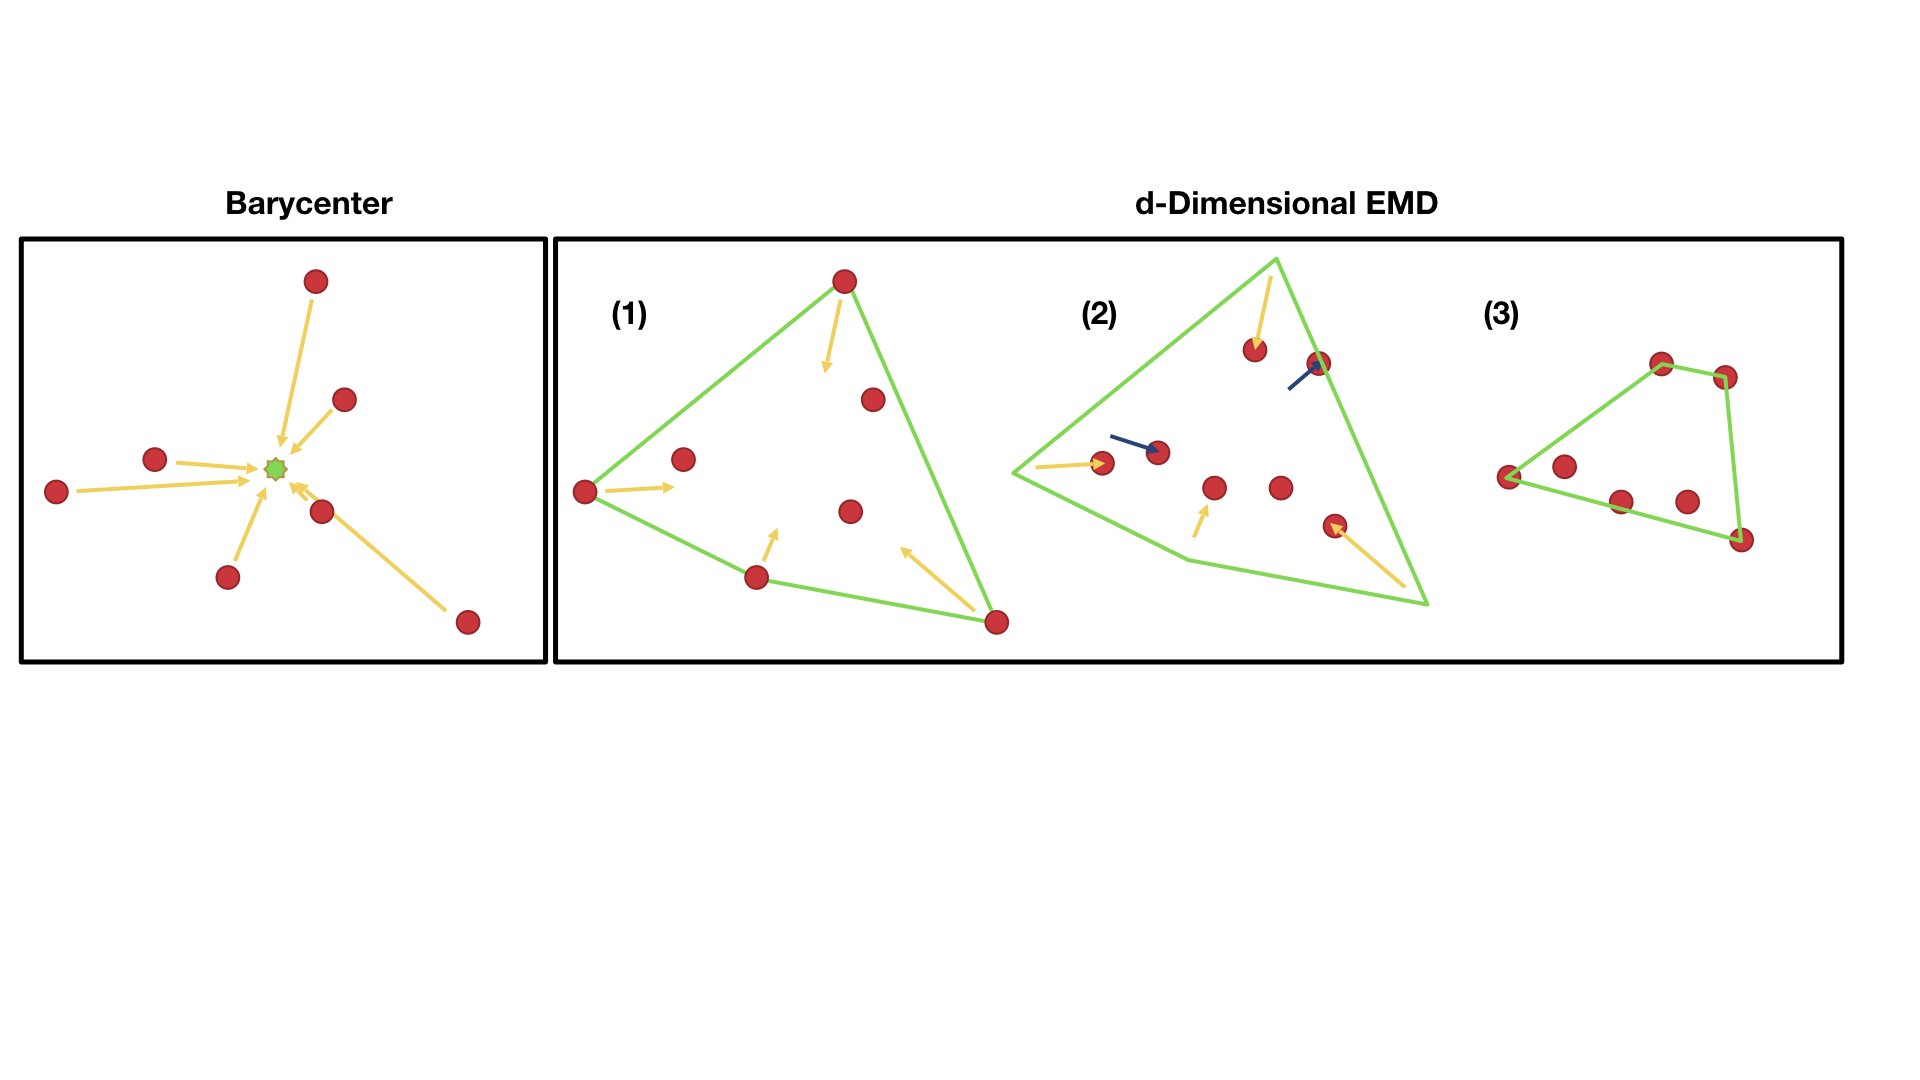
\includegraphics[trim={0 14.5cm 2cm 5cm},clip,width=\textwidth]{figs/demd_abstract.png}
    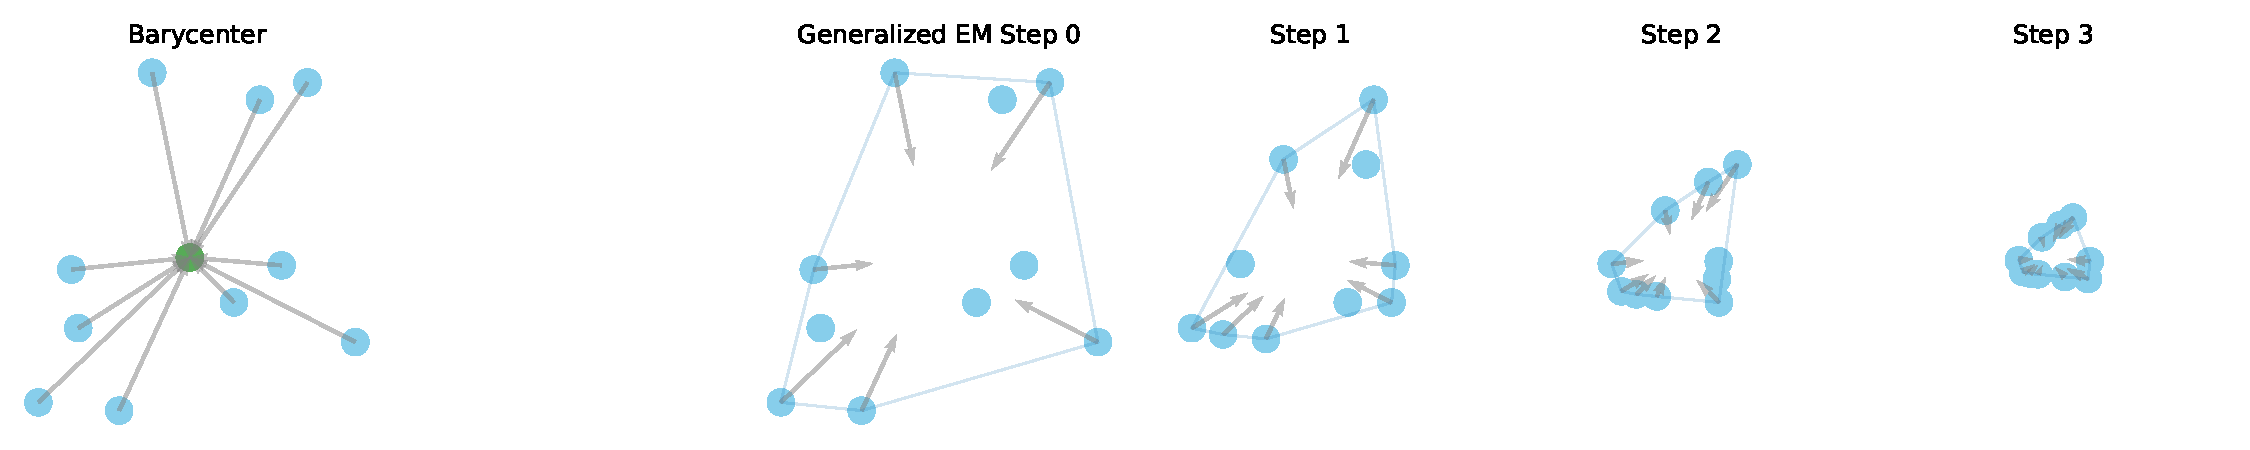
\includegraphics[width=0.95\textwidth]{chap5/bary-gem-step.pdf}
    \caption{({\em Left}) Barycenter approaches identify a center (green) and move samples of interest (blue) toward it along the coupling path (grey). ({\em Right}) Our approach identifies ``support" points that lie within the convex hull,  and only those points are moved in a descent direction. The support points are those that contribute to the objective functional, and it is known (see Theorem 2.2 of~\citep{kline2019properties}) that they are not interior points of the convex hull.}
    \label{fig:min_demd}
\end{figure*}
